% CHAPTER 3: Positional Encoding
\chapter{Positional Encoding}

I believe that the previous chapter would have provided you a deep insight of how self-attention works. Technically speaking, self-attention is at the heart of the working of a transformer. So understanding that completely is a significant milestone in our journey.

In this chapter, we will be discussing an equally important concept. Since self-attention processes all the words simultaneously, it loses the sequential information of text. This is not good since the sequence is what gives meaning to a text (sentence or paragraph). That is why we use \textbf{positional encoding}.
\begin{figure}[H]
    \centering
    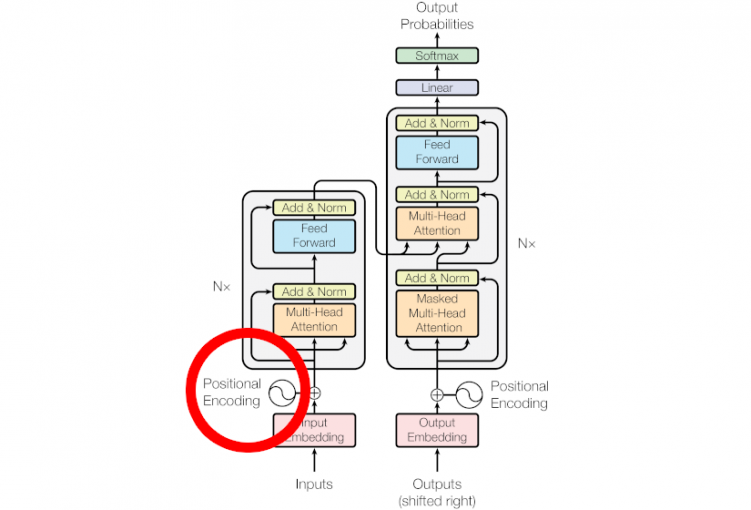
\includegraphics[width=0.5\linewidth]{Positional-encoding/architecture-positional-encoding.png}
    \caption{Positional encoding in transformer architecture}
\end{figure}

% Basic idea
\section{A basic idea}

Again, we will be going forward as if we do not know anything about it and are deriving the concept from first principles. What can be a good way to encode the position of each word? One solution can be to add an extra dimension into the embedding vector and encode the position of the word into it.
\begin{figure}[H]
    \centering
    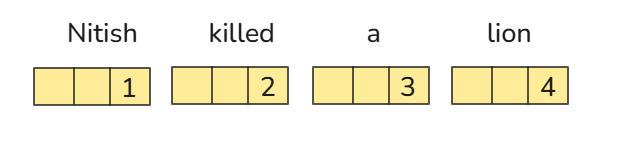
\includegraphics[width=0.75\linewidth]{Positional-encoding/sequential-info.png}
    \caption{Encoding sequential information in the embedding vector}
\end{figure}

But this approach has some problems:
\begin{itemize}
    \item The numbers are unbounded. It can go upto 1000 or 1 lakh for large texts. Deep learning models generally train more efficiently when the input features are properly scaled and have similar magnitudes. The other inputs of the embedding vector are on a different scale than the position.
    \item The position values are discrete. Deep learning models prefer continuous values for efficient training.
\end{itemize}

What if we divided all the positions with the length of the sentence? In that case, all the positions will be within [0, 1] and it will be on the same scale. But this also poses a problem. Different sentences will have different lengths and the positional value assigned to the 2nd word (for example) of one sentence will be different from another. The model will have no idea about the exact position of words in different sentences.
\begin{figure}[H]
    \centering
    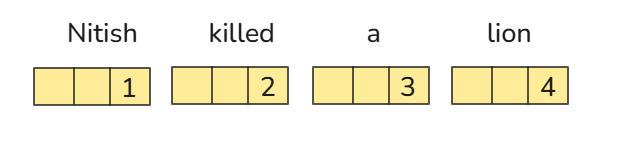
\includegraphics[width=0.75\linewidth]{Positional-encoding/sequential-info.png}
    \caption{Scaled positional values}
\end{figure}

% Periodic functions
\section{Moving on to periodic functions}

What if we used periodic functions for this task? A good function can be $sin(x)$, where $x$ is the position of the word. This solves 2 things:
\begin{itemize}
    \item It provides a bound to the values - [-1, 1]
    \item All the values are continuous
\end{itemize}

But there is a big problem in using this approach and I hope that you are able to figure this out. The problem arises from periodicity (which essentially solved our problem!). Since $sin(x)$ is periodic, the positional values of 2 words can be the same. This is not feasible since the model will not be able to distinguish which comes earlier.

A better version will be to use 2 values instead of one - $sin(x)$ and $cos(x)$. This would reduce the chance of a positional value being repeated. But still there remains a chance of repetition. So instead of using a single pair, we use multiple pairs of $sin(nx)$ and $cos(nx)$ values. Over here, $n$ denotes frequency. This significantly reduces the chance of repetition of any positional value.

The positional values are a vector of the same dimension as the embedding vector. The embedding and the position vectors are added to obtain a final vector, which is then passed on to the self-attention block.

% Expression for PE
\section{The original expression for positional encoding}

According to the paper on transformers, the expression for positional encoding is:
\begin{align}
    PE(pos, 2i) &= sin\left (\frac{pos}{10,000^\frac{2i}{d_{model}}}\right)\\
    PE(pos, 2i+1) &= cos\left (\frac{pos}{10,000^\frac{2i}{d_{model}}}\right)
\end{align}

PE - positional encoding\\
$d_{model}$ - dimension of the embedding vector\\
pos - position of word
i - position in positional encoding vector. Ranges from $[0, \frac{d_{model}}{2} - 1]$

Before moving on to some discussion about the expression, it would be good if we apply this on a sentence to calculate the positional encoding. This would provide us some confidence moving forward.

Consider the sentence: \textit{River bank flows}. Let us consider that the embedding vector for this sentence is 6-dimensional. Hence, i ranges from [0, 2]. We will calculate the positional encoding for the word \textit{river}.
\begin{enumerate}
    \item \textbf{River:} pos = 0
    \begin{itemize}
        \item i = 0:\\
        PE(0, 0) = $sin\left(\frac{0}{10,000^\frac{2(0)}{6}}\right) = 0$\\
        PE(0, 1) = $cos\left(\frac{0}{10,000^\frac{2(0)}{6}}\right) = 1$
        \item i = 1:\\
        PE(0, 2) = $sin\left(\frac{0}{10,000^\frac{2(1)}{6}}\right) = 0$\\
        PE(0, 3) = $cos\left(\frac{0}{10,000^\frac{2(1)}{6}}\right) = 1$
        \item i = 2:\\
        PE(0, 4) = $sin\left(\frac{0}{10,000^\frac{2(2)}{6}}\right) = 0$\\
        PE(0, 5) = $cos\left(\frac{0}{10,000^\frac{2(2)}{6}}\right) = 1$
    \end{itemize}
\end{enumerate}

Hence, \textbf{PE(river) = [0, 1, 0, 1, 0, 1]}. Like this, the PE of all the words can be calculated.

% Multiple frequencies
\section{Why multiple frequencies?}

Over here, the frequency is $\omega_i = 10,000^{-\frac{2i}{d_{model}}}$. But what is special about this frequency? On closer inspection, we see that it forms a geometric progression. The PE for higher frequencies (low i) vary rapidly, whereas PE for lower frequencies vary slowly. Hence, \textit{high-frequency dimensions} distinguish nearby words (since they occur more frequently), whereas \textit{low-frequency dimensions} encode long-range position (sentences and paragraphs). This captures the hierarchy of a text.

This is similar to binary representation of digits
\begin{figure}[H]
    \centering
    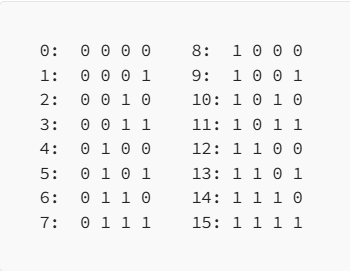
\includegraphics[width=0.4\linewidth]{Positional-encoding/binary-representation.png}
    \caption{Binary representation of digits}
\end{figure}

Notice the pattern in how each bit (column) changes:
\begin{itemize}
    \item The rightmost bit (Least Significant Bit) alternates with every number (frequency: 1/2)
    \item The second bit from the right alternates every two numbers (frequency: 1/4)
    \item The third bit alternates every four numbers (frequency: 1/8) And so on…
\end{itemize}

This pattern of different frequencies is the key to positional encoding. But instead of using discrete bits, we use something smoother: sine and cosine waves.

% Relative positioning
\section{Capturing relative positioning of words}

Consider these sentences:
\begin{itemize}
    \item The cat sat on the mat.
    \item Yesterday the cat sat on the mat.
\end{itemize}

The relationship between cat and sat is the same in both sentences even though their absolute positions differ. A model should ideally learn: \textit{This word is 1 position after that word} (meaning of sequences) rather than \textit{This word is at position 7}. In other words, it should capture the \textbf{relative positioning} of words.

Let us see how our setup captures the relative positioning of words. Let's ignore the full PE for a moment and look at a single sine-cosine pair.
\[
PE(pos)=
\begin{bmatrix}
\sin(\omega\, pos)\\
\cos(\omega\, pos)
\end{bmatrix}
\]

where \(\omega\) is some frequency.

Now suppose we move \(k\) positions ahead in the sequence. The new encoding becomes
\[
PE(pos+k)=
\begin{bmatrix}
\sin(\omega(pos+k))\\
\cos(\omega(pos+k))
\end{bmatrix}
\]

Using the angle addition formulas:
\[
\sin(\omega(pos+k))
=
\sin(\omega pos)\cos(\omega k)
+
\cos(\omega pos)\sin(\omega k)
\]

\[
\cos(\omega(pos+k))
=
\cos(\omega pos)\cos(\omega k)
-
\sin(\omega pos)\sin(\omega k).
\]

Rearranging into matrix form:

\[
\begin{bmatrix}
\sin(\omega(pos+k))\\
\cos(\omega(pos+k))
\end{bmatrix}
=
\begin{bmatrix}
\cos(\omega k) & \sin(\omega k)\\
-\sin(\omega k) & \cos(\omega k)
\end{bmatrix}
\begin{bmatrix}
\sin(\omega pos)\\
\cos(\omega pos)
\end{bmatrix}
\]

\[ \implies
PE(pos+k)
=
M_k\,PE(pos)
\]

where
\[
M_k=
\begin{bmatrix}
\cos(\omega k) & \sin(\omega k)\\
-\sin(\omega k) & \cos(\omega k)
\end{bmatrix}.
\]

Notice something remarkable. The matrix \(M_k\) depends only on the offset \(k\). It does \textbf{not} depend on the absolute position \(pos\). So if 2 words are always 3 positions apart, the same transformation converts the positional encoding of the first word into that of the second, regardless of where they occur in the sentence.

\section{A nice visualization}

Consider a sentence having 100 words. The embedding vector of each word is 128 dimensional. We calculate the positional encoding vectors of each of the words and plot a heat map of \textit{position vs dimension}.
\begin{figure}[H]
    \centering
    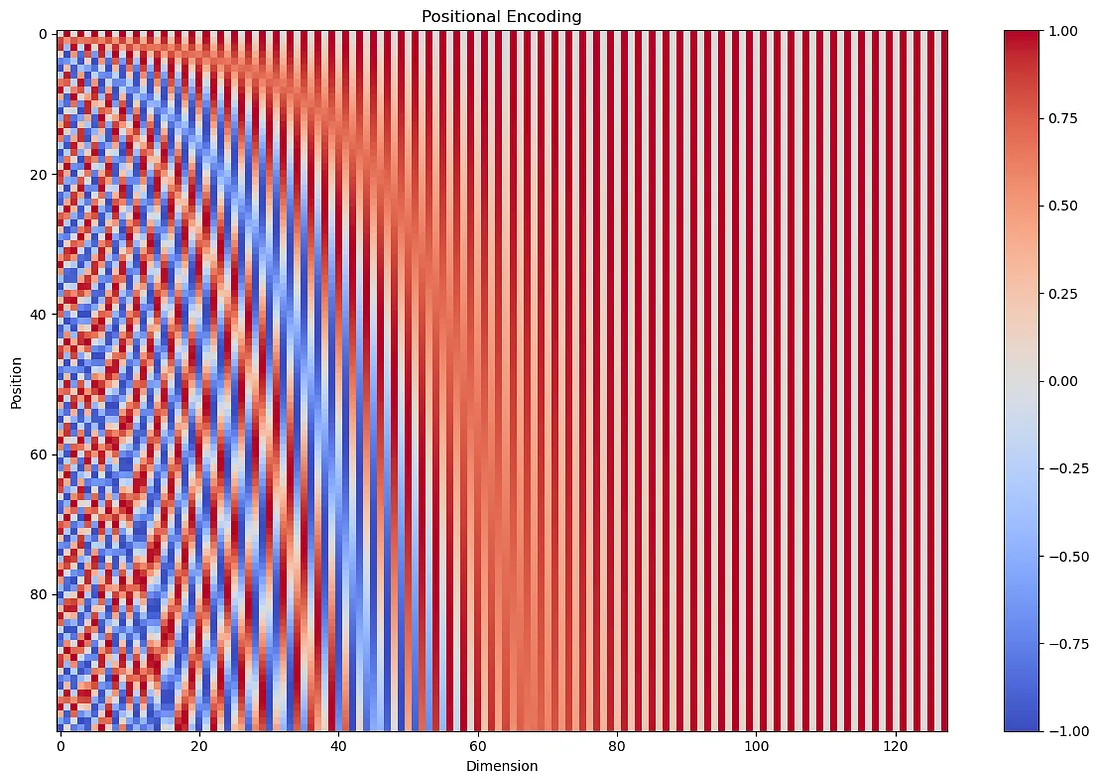
\includegraphics[width=0.6\linewidth]{Positional-encoding/positional-encoding-heatmap.png}
    \caption{Heat map of positional encoding vectors}
\end{figure}

Some key observations:
\begin{itemize}
    \item As we move down the rows (increasing positions), we see patterns of color changes, similar to how bits flip in binary counting.
    \item The leftmost columns (lower dimensions) change rapidly, like the least significant bits in binary.
    \item The rightmost columns (higher dimensions) change more slowly, analogous to the most significant bits in binary.
\end{itemize}